\chapter{Arbeitspunkt-Regelung}\label{cha:apr}

Nachdem im letzten Kapitel die Modellierung des Gesamtsystems erläutert wurde, stellt sich nun Frage, wie sich das System regeln lässt. Dabei geht es einerseits um die Regelung an den 4 Arbeitspunkten \secref{sec:aps} sowie um \traj n, die das \dpd\ von einem \ap\ in einen anderen überführen.

\section{Vorgehen}%\label{sec:}

Beim Reglerentwurf wird zunächst dem Vorgehen vergangener Arbeiten gefolgt. 

\subsection{\lin}

Da das \zrm\ des \spds s \eqref{eq:zrm} nicht-linear ist, muss es um jeden \ap\ linearisiert werden, bevor lineare Regelungsmethoden angewandt werden können. 
\begin{align}
	\mat{A} &= \left. \frac{\partial \vef(\vex,u_R)}{\partial \vex} \right|_{\vex=\vexr}  
		= \left. \begin{bmatrix}
		0 & 1 & 0 & 0 & 0 & 0 \\
		0 & \partiald{a_2(\vex)}{\xop} & \partiald{a_2(\vex)}{\phe} & \partiald{a_2(\vex)}{\phep} & \partiald{a_2(\vex)}{\phz} & \partiald{a_2(\vex)}{\phzp} \\
		0 & 0 & 0 & 1 & 0 & 0 \\
		0 & \partiald{a_4(\vex)}{\xop} & \partiald{a_4(\vex)}{\phe} & \partiald{a_4(\vex)}{\phep} & \partiald{a_4(\vex)}{\phz} & \partiald{a_4(\vex)}{\phzp} \\
		0 & 0 & 0 & 0 & 0 & 1 \\
		0 & \partiald{a_6(\vex)}{\xop} & \partiald{a_6(\vex)}{\phe} & \partiald{a_6(\vex)}{\phep} & \partiald{a_6(\vex)}{\phz} & \partiald{a_6(\vex)}{\phzp} \\
	\end{bmatrix} \right._{\vex=\vexr}  \\
	\mat{B} &= \left. \frac{\partial \vef(\vex_R,u)}{\partial u} \right|_{u=u_R}
	= \ve{b}(\vexr) = \begin{bmatrix}
		0 \\ b_2(\vexr) \\ 0 \\  b_4(\vexr) \\ 0 \\  b_6(\vexr)
	\end{bmatrix}
\end{align}
Somit ergeben sich für jeden \ap\ unterschiedliche Systemmatrizen \mat{A} und Eingangsmatrizen \ve{B}. Beim \bss\ fällt zusätzlich die zweite Zeile und die zweite Spalte (bis auf die 1) weg, da dort $a_2=0$ ist und keine Abhängigkeit von \xop\ besteht (siehe \tabref{tab:abh}), außerdem ist $b_2=1$.
Die Ausgangsmatrix \mat{C} ist immer gleich, da die Ausgangsgleichung \eqref{eq:hx} linear ist.


\subsection{Eigenwerte}

Anhand der \ewe\ können Aussagen über die Dynamik eines Systems getroffen werden. 
Beim \bss\ gibt es aufgrund der zweifachen Integration des Eingangs \xopp\ stets zwei \ewe\ in 0. 
Mit den Apprich-Parametern ergeben sich folgende \ewe:
\begin{table}[htbp]
	\centering
		\begin{tabular}[t]{cccc}
			\toprule
			\ape & \apz & \apd & \apv \\
			\midrule
			$0$	&	$0$	&	$0$	&	$0$	\\
			$0$	&	$0$	&	$0$	&	$0$	\\
			$-0.2972 +11.4177\iu$ &    $7.8028						$	&	  $6.8596							$	&   $11.1308$	\\
			$-0.2972 -11.4177\iu$ &   $-7.9367						$	&   $-7.2314					$		&  $-11.7251$	\\
			$-0.0418 + 4.8515\iu$ &   $-0.1858 + 7.0392\iu$	&  $-0.0669 + 7.8676\iu$	&  $  4.8089$	\\
			$-0.0418 - 4.8515\iu$ &   $-0.1858 - 7.0392\iu$	& $ -0.0669 - 7.8676\iu	$	&  $ -4.8926$	\\
			\bottomrule
		\end{tabular}
	\caption{\ewe\ des \bss s (Parameter: Apprich)}
	\label{tab:ewappr}
\end{table}

Im \ap\ 1 ergeben sich zwei konjugiert-komplexe Polpaare, die sich physikalisch mit der Schwingung der beiden Pendel begründen lassen. Sie befinden sich aufgrund der Dämpfung in der linken s-Halbebene, es ist der einzige stabile \ap. \ap\ 2 und 3 besitzen jeweils ein konjugiert-komplexes Polpaar, da dort das erste \bzw zweite Pendel nach unten zeigt und damit \qq{stabil} ist. Der Realteil ist bei \ap\ 3 deutlich kleiner, was auf die geringere Dämpfung des zweiten Pendelgelenks zurückzuführen ist (siehe \tabref{tab:parappr}). Aufgrund der Instabilität des anderen Pendels ergibt sich jeweils ein positiv reeller \ew. In \ap\ 4 stehen beide Pendel oben, weswegen es dort zwei \ewe\ in der rechten s-Halbebene gibt.

\begin{table}[htbp]
	\centering
		\begin{tabular}[t]{cccc}
			\toprule
			\ape & \apz & \apd & \apv \\
			\midrule
				$0$	&	$0$	&	$0$	&	$0$	\\
				$0$	&	$0$	&	$0$	&	$0$	\\
				$-174.3727$						&	$-172.9211$	&	$-173.2473$						&	$-175.4362$	\\
				$-0.3493$							&	$-0.3494$		&	$0.3471$							&	$0.3471$	\\
				$-0.6385 + 7.1578\iu$	&	$6.7715$		&	$-0.6443 + 7.2040\iu$	&	$6.7469$	\\
				$-0.6385 - 7.1578\iu$	&	$-7.6900$ 	&	$-0.6443 - 7.2040\iu$ &	$-7.6570$ \\
			\bottomrule
		\end{tabular}
	\caption{\ewe\ des \bss s (Parameter: Ribeiro)}
	\label{tab:ewribe}
\end{table}

Mit den neuen Parametern (Ribeiro) ergibt sich ein anderes Bild (siehe \tabref{tab:ewribe}).
Bei \ap\ 1 und 2 verschwindet ein Polpaar, welches dem ersten Pendel zugeordnet wurde. Ein sehr schneller \ew\ kommt hinzu, außerdem ein langsamer reeller, der bei \ap\ 3 und 4 positiv ist. 
Die Ursache für diese Änderung liegt vermutlich in der Modellierung der \crb\ (siehe \secref{sec:crb}). Bei der \lin\ um die Ruhelage wird die Annäherungsfunktion der \mrm{signum}-Funktion um 0 linearisiert, wo sie sehr steil ist. Dies resultiert in einer sehr hohen Dämpfung. Daher ist es sinnvoll, die \crb\ der Pendelstäbe für den AP-Reglerentwurf zu vernachlässigen.
Wird die \crb\ zu 0 gesetzt, ergeben sich prinzipiell ähnliche Werte wie in \tabref{tab:ewappr}.


\subsection{Steuerbarkeit und Beobachtbarkeit}

Voraussetzung für eine Regelung ist die Steuerbarkeit des Systems. Diese kann für lineare Systeme oder linearisierte Systeme an einem \ap\ mit dem Steuerbarkeitskriterium nach Kalman überprüft werden \cite{AdamyRT2}. Außerdem sollte ein System beobachtbar sein, falls nicht alle Zustände bekannt sind und daher über einen Beobachter ermittelt werden.

Das \spds\ (\bss) ist an allen 4 \ap en vollständig steuer- und beobachtbar.


\subsection{Zustandsregler}

Die \aprg\ wird mit einem \zsr\ realisiert. Die Verstärkung $K$ wird durch Lösen des LQ-Problems ermittelt \cite{AdamyRT2}. Parameter für den Entwurf sind somit die Matrix \mat{Q} zur Bewertung der Zustände und $R$ für die Stellgröße. 

Für jeden \ap\ muss ein eigener Regler entworfen werden. 




\section{Aufbau in \Simulink}



\section{Implementierung in \Matlab}



\section{Anfangswert-Tests}

\begin{figure}
	\centering
	\begin{minipage}[t]{0.45\linewidth}
		\centering
		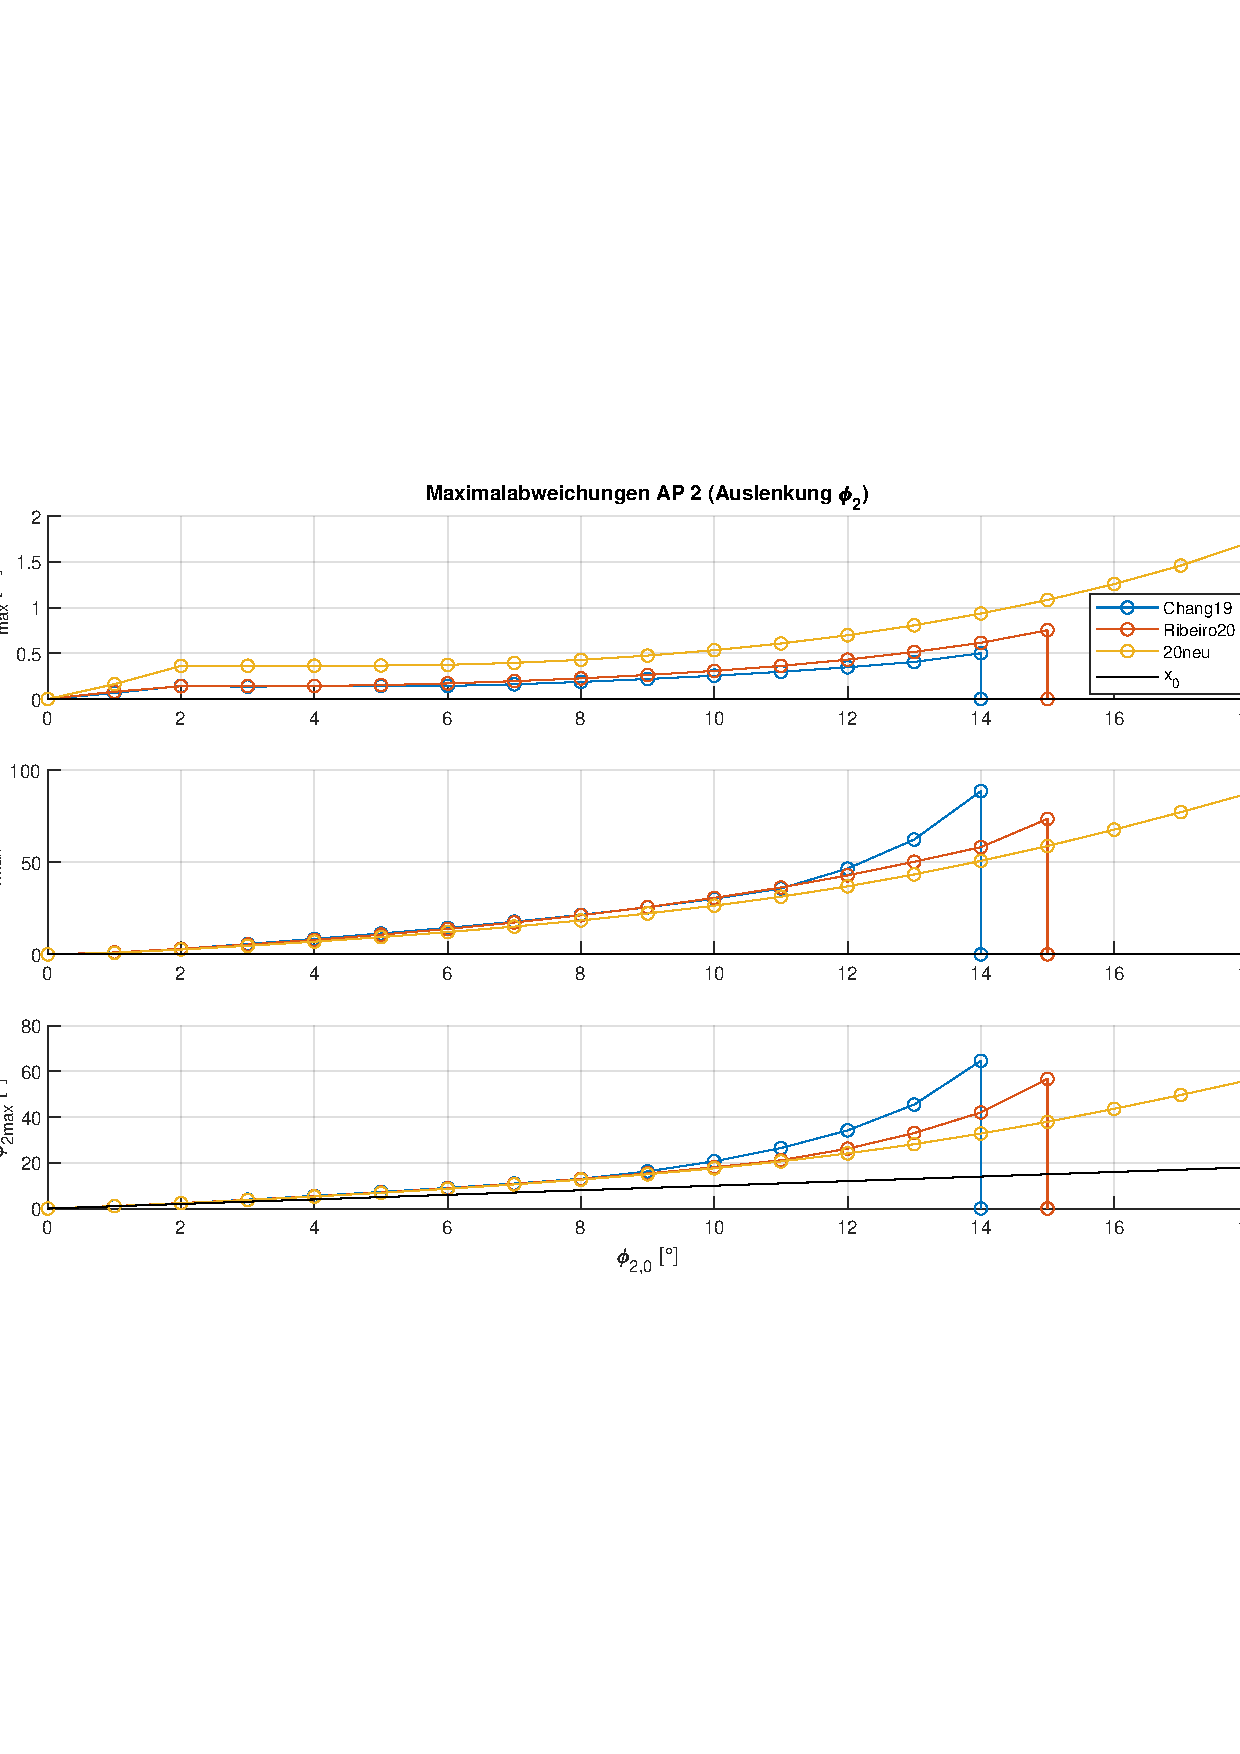
\includegraphics[scale=0.5]{Bilder/Parameter neu (Ribeiro) Creg off/AP2.pdf}
		%\caption{\ap  2}
		\label{fig:ap2}
	\end{minipage}
	\hfill
	\begin{minipage}[t]{0.45\linewidth}
		\centering
		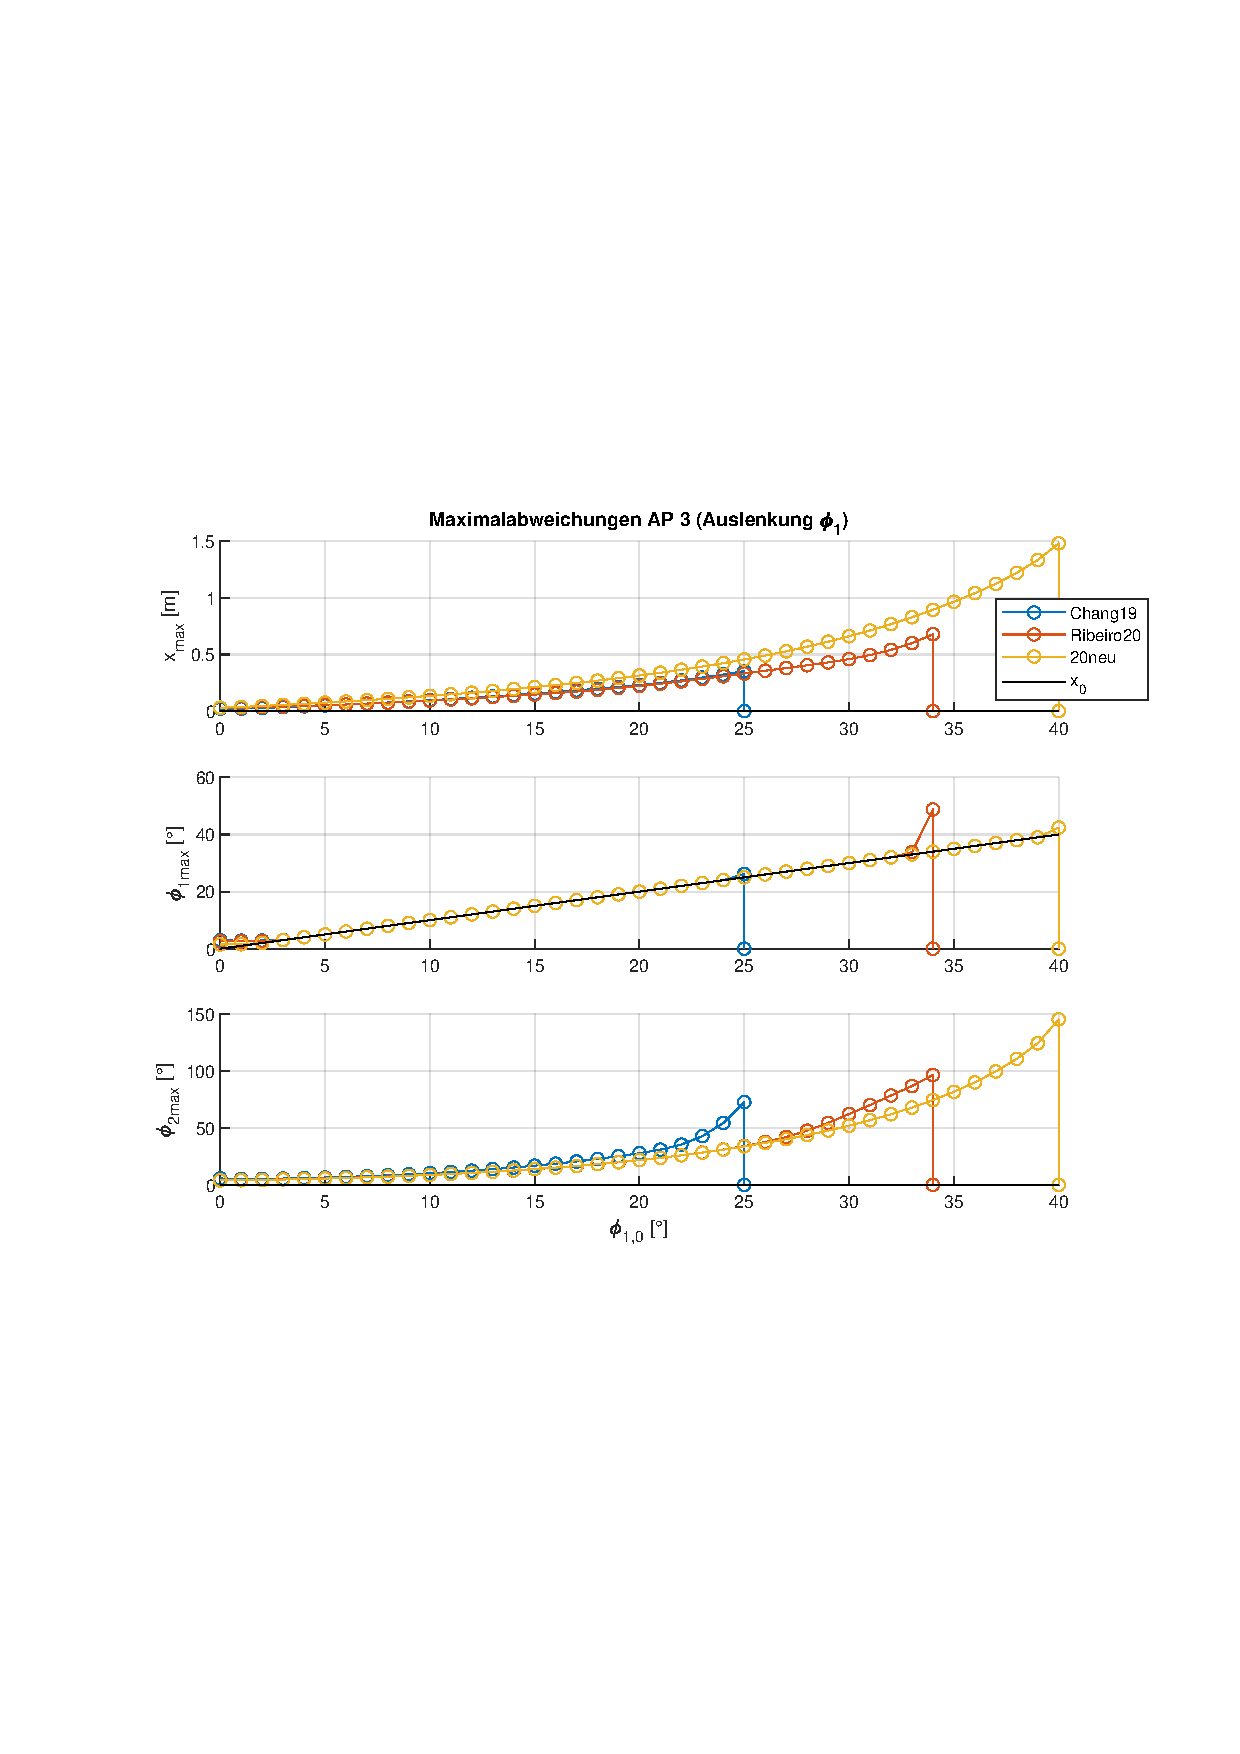
\includegraphics[scale=0.5]{Bilder/Parameter neu (Ribeiro) Creg off/AP3.pdf}
		%\caption{\ap  3}
		\label{fig:ap3}
	 \end{minipage}
	\\
	\begin{minipage}[t]{0.45\linewidth}
		\centering
		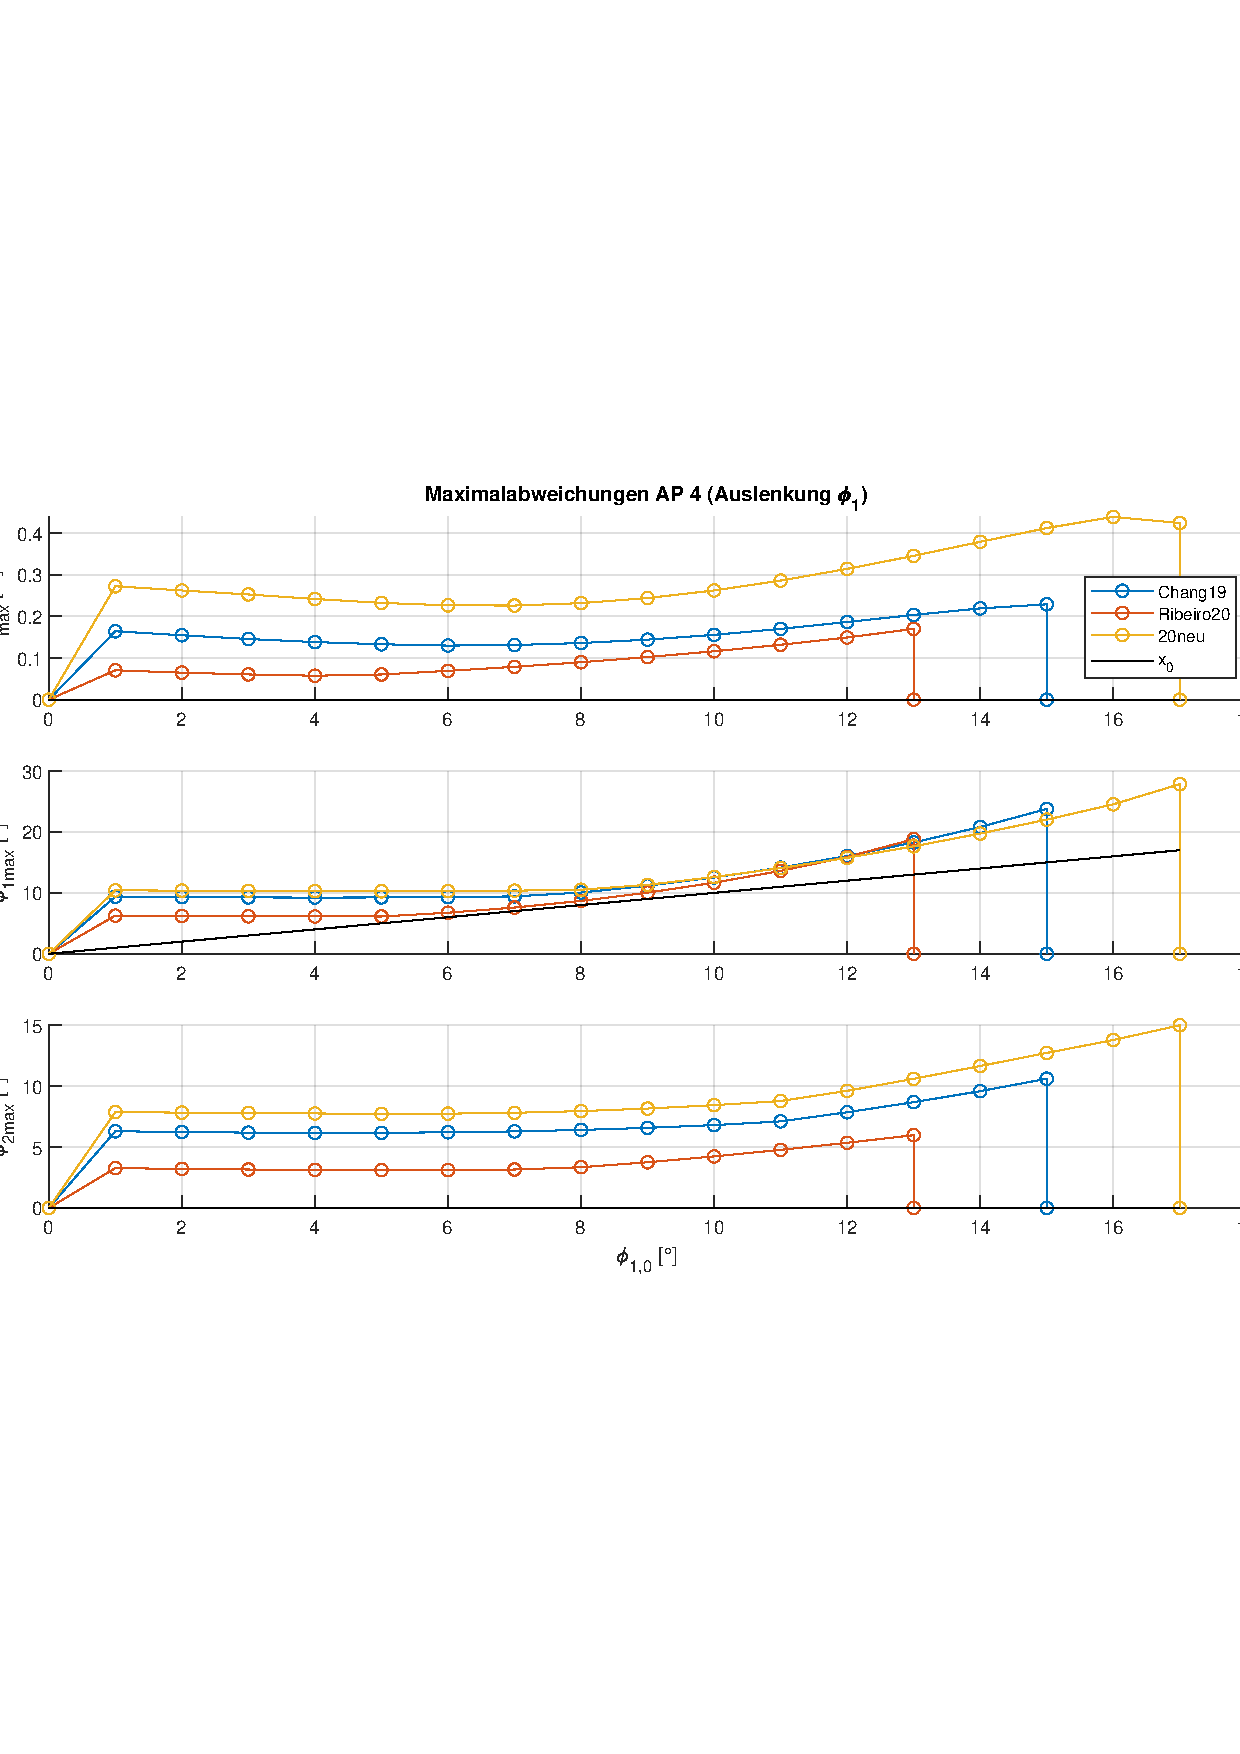
\includegraphics[scale=0.5]{Bilder/Parameter neu (Ribeiro) Creg off/AP41.pdf}
		%\caption{\ap  3}
		\label{fig:ap3}
	 \end{minipage}
	\hfill
	\begin{minipage}[t]{0.45\linewidth}
		\centering
		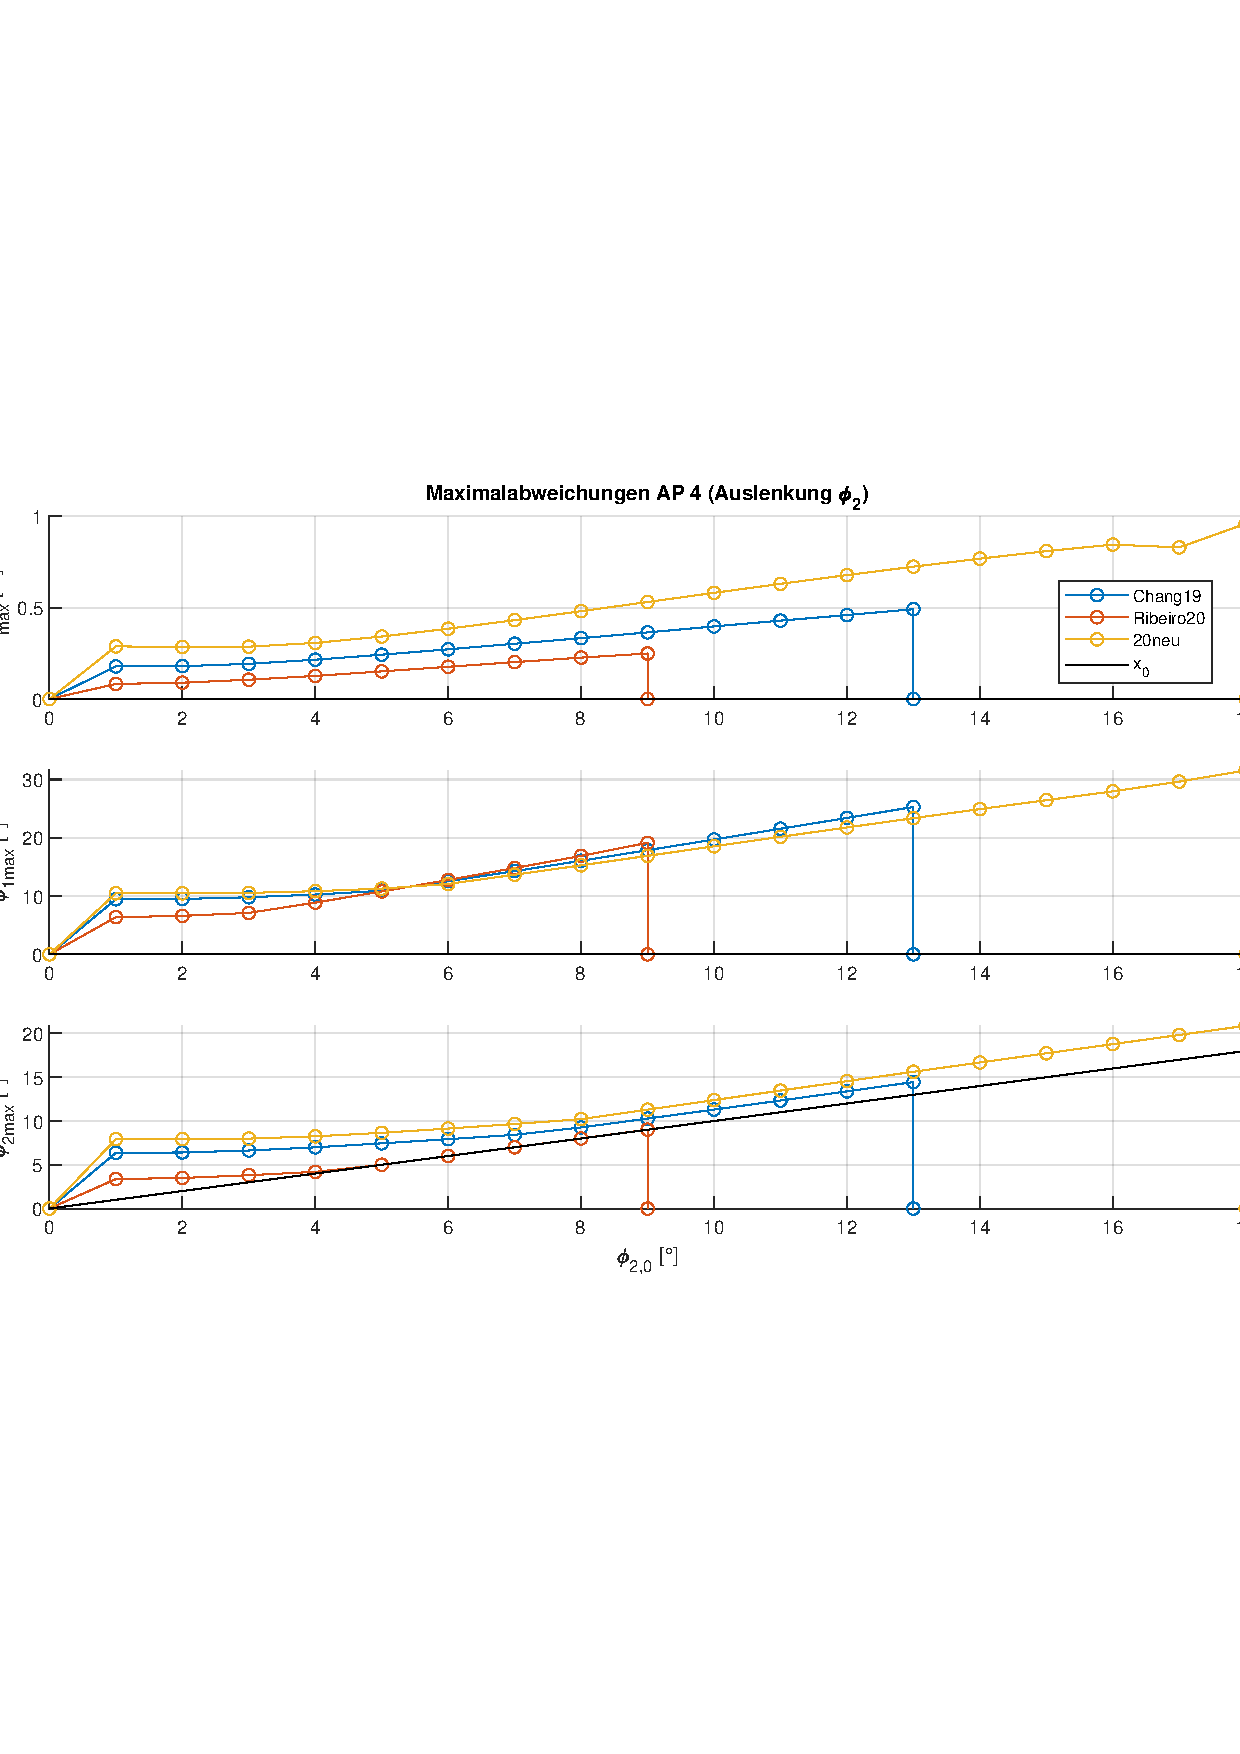
\includegraphics[scale=0.5]{Bilder/Parameter neu (Ribeiro) Creg off/AP42.pdf}
		%\caption{\ap  3}
		\label{fig:ap3}
	 \end{minipage}
	\caption{Vergleich QR-Parameter (System Ribeiro)}
%\vspace{15pt}
\end{figure}




\section{QR Parameter Tests}



\section{System Parameter Tests}



